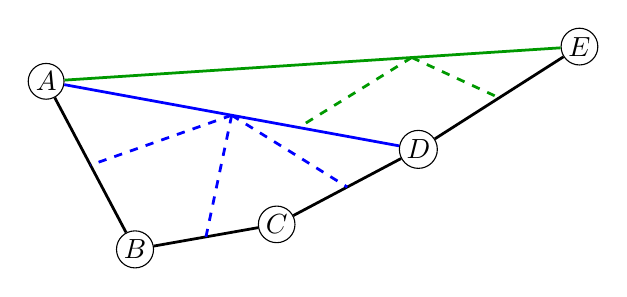
\begin{tikzpicture}
  \node (A) at (0bp,75bp)     [draw, circle, inner sep=1pt] {$A$};
  \node (B) at (32bp,14.5bp)  [draw, circle, inner sep=1pt] {$B$};
  \node (C) at (83bp,23.5bp)  [draw, circle, inner sep=1pt] {$C$};
  \node (D) at (134bp,50.5bp) [draw, circle, inner sep=1pt] {$D$};
  \node (E) at (192bp,87.5bp) [draw, circle, inner sep=1pt] {$E$};

  \draw (A) -- (B) [line width=1pt, black] coordinate[pos=.5] (AB);
  \draw (B) -- (C) [line width=1pt, black] coordinate[pos=.5] (BC);
  \draw (D) -- (C) [line width=1pt, black] coordinate[pos=.5] (CD);
  \draw (D) -- (E) [line width=1pt, black] coordinate[pos=.5] (DE);

  \draw (A) -- (D) [line width=1pt, blue] coordinate[pos=.5] (ADdown) coordinate[pos=.7] (ADup);

  \draw (ADdown) -- (AB) [line width=1pt, blue, dashed];
  \draw (ADdown) -- (BC) [line width=1pt, blue, dashed];
  \draw (ADdown) -- (CD) [line width=1pt, blue, dashed];

  \draw (A) -- (E) [line width=1pt, black!40!green] coordinate[pos=.7] (AE);

  \draw (AE) -- (ADup) [line width=1pt, black!40!green, dashed];
  \draw (AE) -- (DE) [line width=1pt, black!40!green, dashed];
\end{tikzpicture}
